\ffigbox[\FBwidth]{%
\caption{\centering Complémentaire du graphe \(C_5\)}\label{Fig:exam_blanc_ex_5_2_b}
}{
    \fbox{
        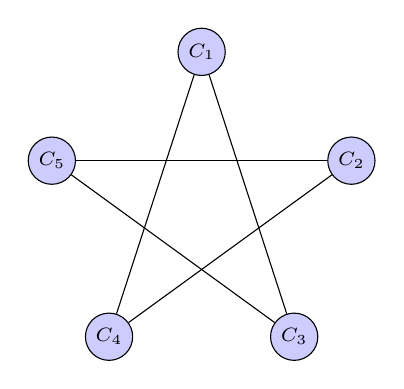
\begin{tikzpicture}[scale=1, main node/.style={circle, draw, fill=blue!20, inner sep=1pt, font=\scriptsize, minimum size=6mm}]
            % les sommets initiaux
            \node[main node] (C1) at (90:2)  {\(C_1\)};
            \node[main node] (C2) at (18:2)  {\(C_2\)};
            \node[main node] (C3) at (-54:2) {\(C_3\)};
            \node[main node] (C4) at (-126:2){\(C_4\)};
            \node[main node] (C5) at (-198:2){\(C_5\)};

            % les aretes
            \draw[] (C1) -- (C3);
            \draw[] (C1) -- (C4);
            
            \draw[] (C2) -- (C4);
            \draw[] (C2) -- (C5);
            
            \draw[] (C3) -- (C5);
        \end{tikzpicture}
    }
}